
%************************************************************************
\section{Introduction}
\label{sec:intro}
%************************************************************************

We study the SysML model of the ceiling speed monitoring (CSM)
function using the Tina model-checking toolbox. We base our analysis
on a model provided by the University of Bremen that was slightly
extended with information on the environment of the system. The same
function was studied by the University of Rostock using a software
testing approach.

The cornerstone of our approach is an automatic transformation from
SysML models to Time Petri Net. We can then use the resulting formal
model to check several temporal logic formulas.


%************************************************************************
\section{Model Transformation from UML to Time Petri Nets}
\label{sec:uml}
%************************************************************************

This section gives some background information on the translation from
SysML to Time Petri Net (TPN) used in our study. This transformation
is based on a mapping from \uml (Unified Modeling Language) to TPN
described in the PhD thesis of Ning Ge~\cite{Ge2014}. The
transformation can also take into account realtime properties defined
using the \marte profile (Modeling and Analysis of Real Time and
Embedded systems).

By nature, \uml is intended to be a general purpose modeling language
and, as such, it integrates different modeling viewpoints through the
definition of a large class of diagram elements. In this work, we
select a core subset of \uml diagrams and diagram elements for
modeling real-time software architecture and behavior, and focus on
the semantic mapping from the \uml model to the verification model.

We briefly describe the different elements supported in our
translation.

\subsection{Architecture Model}
The purpose of architecture model is to connect different sub-system
behavior models and create a system-level model, by means of
communication media. The objective of the mapping is to replace each
architecture model's entities by its relevant behavior model.  We rely
on the composite structure diagram as the architecture model.
Composite structure diagrams specify the internal structure of a
class, including its interaction points to other parts of the system,
and the architecture of all parts managed by this class. They are used
to explore run-time instances of interconnected instances
collaborating over communications links.

\subsection{Behavioral Model}
The mapping semantics for behavioral model covers both activity and
state machine diagrams.

Activity diagrams express the coordination between lower-level
behaviors using constraints on the possible sequence of actions. In
this context, actions can be triggered because other actions finish
executing; because objects and resources become available; or because
external events occur. The main elements in \uml activity diagram
behavior model are control nodes, actions, objects, and connection
elements.

% The behavior of state machines is modeled as a traversal of a graph of
% state nodes interconnected by one or more joined transition arcs that
% are triggered by the dispatching of series of (event)
% occurrences. During this traversal, the state machine executes a
% series of activities associated with various elements of the state
% machine.

\subsection{Principles of Semantic Mapping}

The mapping from \uml-\marte to TPN preserves the semantics of the
input language. A particularity of the approach is that, for
efficiency reason, the transformation is driven by the set of
real-time properties that should be checked on the resulting
model. For instance, in order to reduce the size of the state space
explored during the verification phase, the behavior of some elements
irrelevant to the target property can be abstracted. The
transformation conforms to the following principles:
%%
\begin{itemize}
\item The resulting \tpn models should be easy to analyze, meaning
  that the semantics mapping should allow the use of high-level
  abstraction methods during model checking.
\item In order to keep the transformation simple, we use a
  compositional approach where the resulting system is obtained by
  composing the interpretation of all its elements. Then, to optimize
  the result, we apply a state space reduction phase that eliminates
  the elements irrelevant to the verification.
\end{itemize}



%************************************************************************
\section{Model Transformation from SysML to Time Transition System}
\label{sec:sysml}
%************************************************************************

Instead of the thirteen diagrams available in \uml 2, the \sysml
includes only nine diagrams, including:
%%
\begin{itemize}
\item
the Block Definition Diagram (BDD), replacing the \uml 2 class diagram
\item
the Internal Block Definition Diagram (IBDD), replacing the \uml 2 composite structure diagram
\item
the Parameter diagram, a \sysml extension to analyze critical system parameters
\item
the Package diagram remained unchanged. 
\end{itemize}

The behavior diagrams includes:
\begin{itemize}
\item
the activity diagram, slightly modified from \uml 2
\item
the sequence, state machine, and use case diagrams remain unchanged. 
\end{itemize}

The requirement diagram is a \sysml extension to describe functional, performance, and interface requirements.	

In order to reuse the existing transformation form \uml to
TPN~\cite{Ge2014} to build a mapping from SysML, we have redefined the
mapping semantics for the block diagram as structure models. The
mapping semantics for the activity and state machine diagrams are left
unchanged. Some of the semantics mapping have also been modified in
order to take into account some of the modeling convention adopted in
the OpenETCS project.

Also, the target model is now an extension of Time Petri Net with
priorities and typed variables called TTS, for Time Transition
System. The data handling ability of TTS is used to model the guards
and actions on integer and float variables found in a SysML diagram.


%************************************************************************
\section{Description of the Ceiling Speed Monitoring Model  and its Extension}
\label{sec:csm}
%************************************************************************
The detailed CSM \sysml model is described in \cite{csmwp4} and
available in the 05-Work folders. The model was edited, and later
extended, using Papyrus. The main addition made to the existing model
for the CSM function is the definition of the environment; mainly the
possible actions on the current speed of the train resulting from 
acceleration or deceleration orders. 

The combination of a test environment model and an optional test driver
model provides a deterministic model

\subsection{Description of the Environment Model}
The environment model is defined in the TestEnvironment block. It is
described using a state machine diagram as shown in
Fig. \ref{fig:env}.

\begin{figure}[ht!]
	\centering
	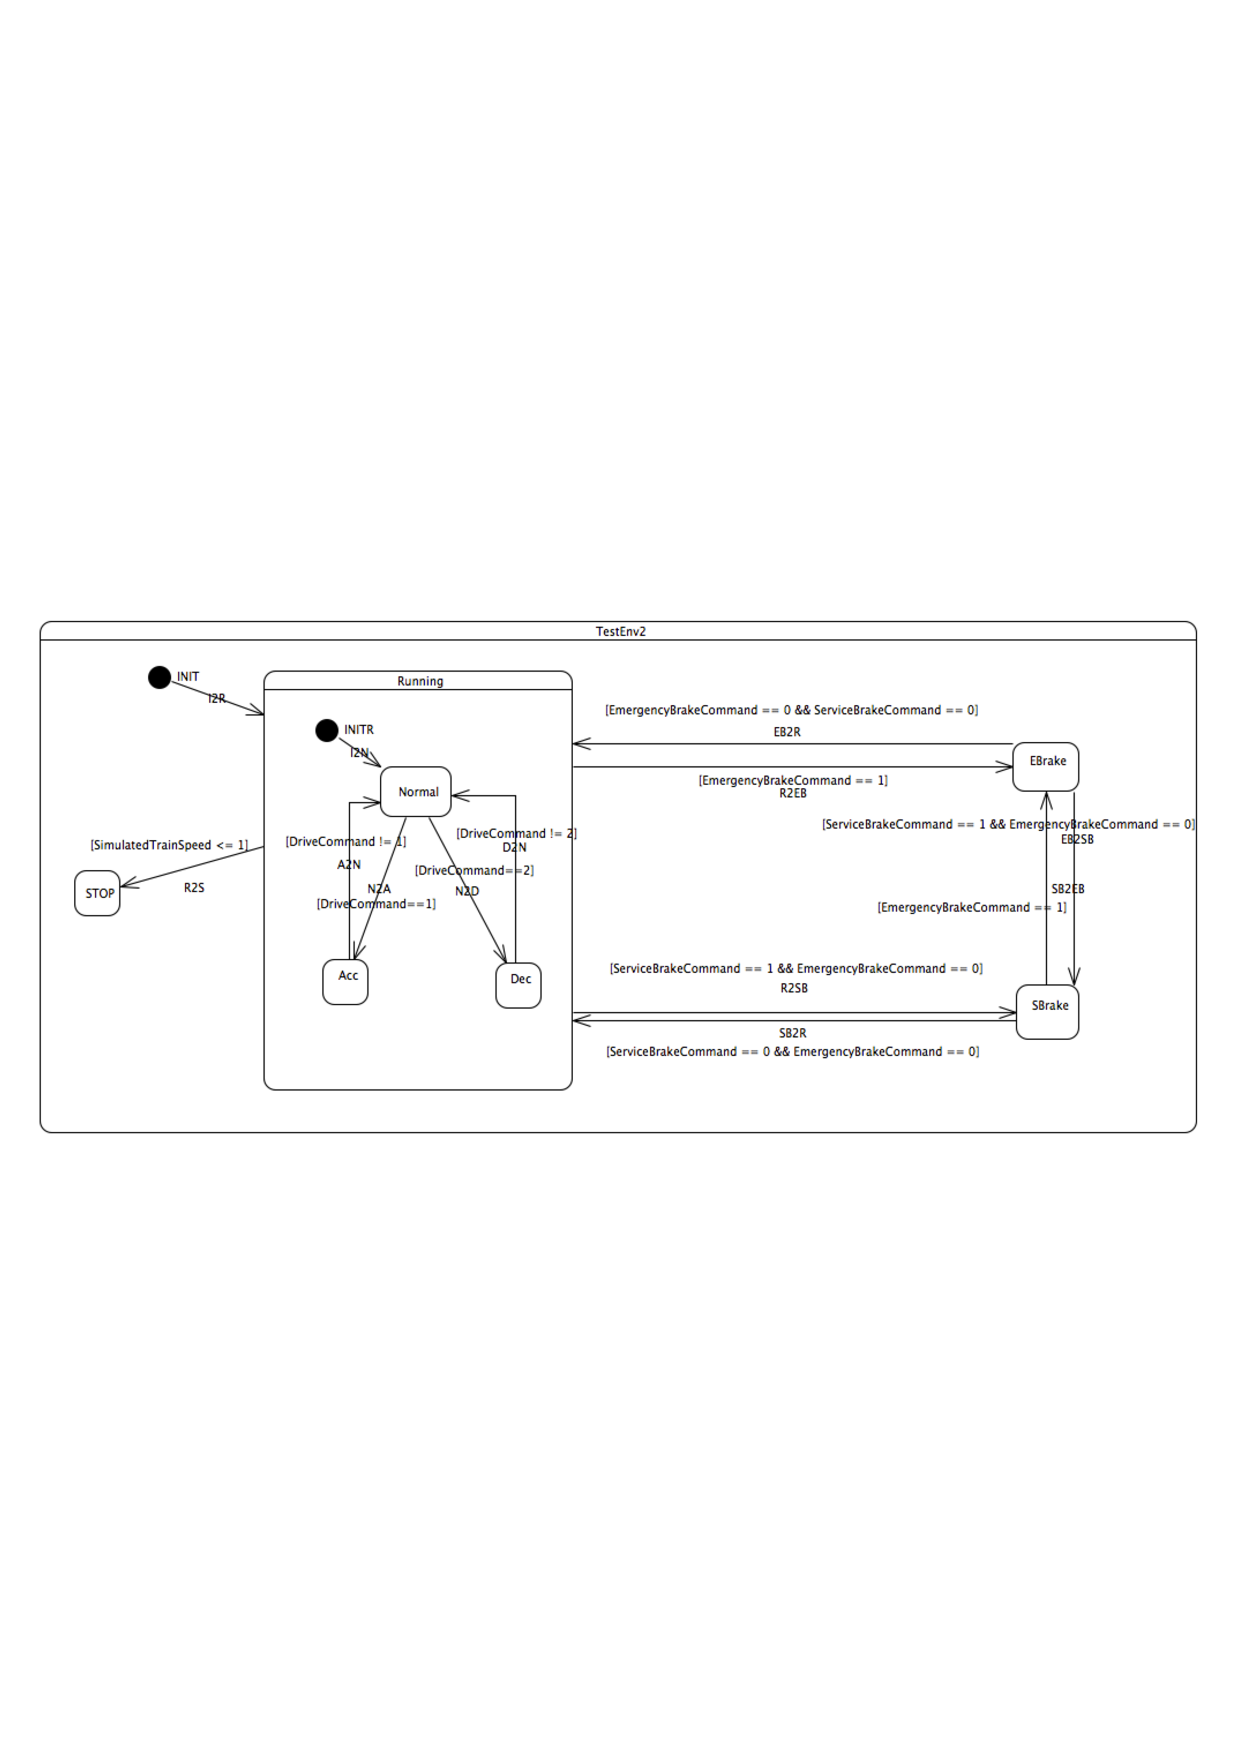
\includegraphics[height=1\textheight]{figures/env}
	\caption{Test Environment Model}
    \label{fig:env}
\end{figure}

The system under test is activated with an initial speed
(SimulatedTrainSpeed) and may enter into the composite state Running.
The Running state encapsulates three possible behavior. Either the
speed remains unchanged (state Normal), or the train accelerates
(state Acc), or the train decelerates (state Dec). The guards defined
on the transitions found inside the composite state Running are
described in Table \ref{tab:runningtr}. The DriveCommand is the
command sent by the driver which contains three modes: keeping speed
(DriveCommand = 0), acceleration (DriveCommand = 1) and Deceleration
(DriveCommand = 2).

\begin{table}[ht!]
	\caption{Transitions between Running States}
	\begin{center}
    \begin{tabular}{|c|c|c|c|}
    \hline
    \backslashbox{To}{From}  & Normal & Acc & Dec \\
    \hline
    Normal &   &  DriveCommand != 1  & DriveCommand != 2\\
    \hline
    Acc  & DriveCommand == 1 & &  \\
    \hline
    Dec  & DriveCommand == 2 & & \\
	\hline
    \end{tabular}
    \end{center}
\label{tab:runningtr}
\end{table} 

The actions on each transition (the "do behaviors") are described in
Table \ref{tab:runningdo}. At the moment we use dummy values for the
acceleration and braking parameters of the train. We have chosen a fix
acceleration of 2 km/h per 100 units of time (\tu) and a constant
braking factor of 2 km/h per 400 \tu.

\begin{table}[ht!]
\footnotesize
	\caption{Do Behaviors in Running States}
	\begin{center}
    \begin{tabular}{|c|c|}
	\hline    
    Normal & \\
	\hline    
    Acc & SimulatedTrainSpeed = SimulatedTrainSpeed + 2; \\
	\hline    
    Dec & SimulatedTrainSpeed = SimulatedTrainSpeed - 2;\\
	\hline
    \end{tabular}
    \end{center}
\label{tab:runningdo}
\end{table} 

The effect of the environment on the system is described by the
transitions between states Running, EBrake (emergency brake), SBrake
(service brake) and STOP (simulatedTrain Speed <= 1). The transition
guards between environment states are described in Table
\ref{tab:envtr}. The transitions are controlled by the commands
EmergencyBrakeCommand and ServiceBrakeCommand generated from the train
control system.

\begin{table}[ht!]
\scriptsize
	\caption{Transitions between Environment States}
	\begin{center}
    \begin{tabular}{|c|c|c|c|c|}
    \hline
    \backslashbox{To}{From}  & Running & EBrake & SBrake & STOP \\
	\hline
	Running & & \begin{tabular}[x]{@{}c@{}}ServiceBrakeCommand == 0 \&\& \\ EmergencyBrakeCommand == 0\end{tabular}  &\begin{tabular}[x]{@{}c@{}}ServiceBrakeCommand == 0 \&\& \\ EmergencyBrakeCommand == 0\end{tabular}     & \\
	\hline
	EBrake &  EmergencyBrakeCommand == 1  & &\begin{tabular}[x]{@{}c@{}}ServiceBrakeCommand == 0 \&\& \\ EmergencyBrakeCommand == 1\end{tabular} & \\
	\hline
	SBrake &  \begin{tabular}[x]{@{}c@{}}ServiceBrakeCommand == 1 \&\& \\ EmergencyBrakeCommand == 0\end{tabular}  & \begin{tabular}[x]{@{}c@{}}ServiceBrakeCommand == 1 \&\& \\ EmergencyBrakeCommand == 0\end{tabular}   & & \\
	\hline
	STOP &  SimulatedTrainSpeed <= 1 & & & \\
	\hline
    \end{tabular}
    \end{center}
\label{tab:envtr}
\end{table} 

The do behaviors in environment states are described in Table
\ref{tab:envdo}. The deceleration of emergency brake is set at 10 km/h
per 200 \tu. The deceleration of service brake is set at 5 km/h per
200 \tu.

\begin{table}[ht!]
  \footnotesize
  \caption{Do Behaviors in Environment States}
  \begin{center}
    \begin{tabular}{|c|c|}
      \hline    
      Running & \\
      \hline    
      EBrake & SimulatedTrainSpeed = SimulatedTrainSpeed - 10; \\
      \hline    
      SBrake & SimulatedTrainSpeed = SimulatedTrainSpeed - 5;\\
      \hline
      STOP & \\
      \hline
    \end{tabular}
  \end{center}
  \label{tab:envdo}
\end{table} 

\subsection{Description of the Driver Model}

In addition to the model of the train behavior we have added a model
of the driver (and of the track description) that can be used to force
a particular scenario. In this context, a scenario is a timed
annotated sequence of acceleration and deceleration orders. One
possible scenario can be obtained using the model defined in the
TestDriver block of Fig. \ref{fig:driver}. This test describes a
situation where the driver accelerates for a time T1 (DriveCommand =
1) before decelerating for a time T2. 

\begin{figure}[ht!]
  \centering
  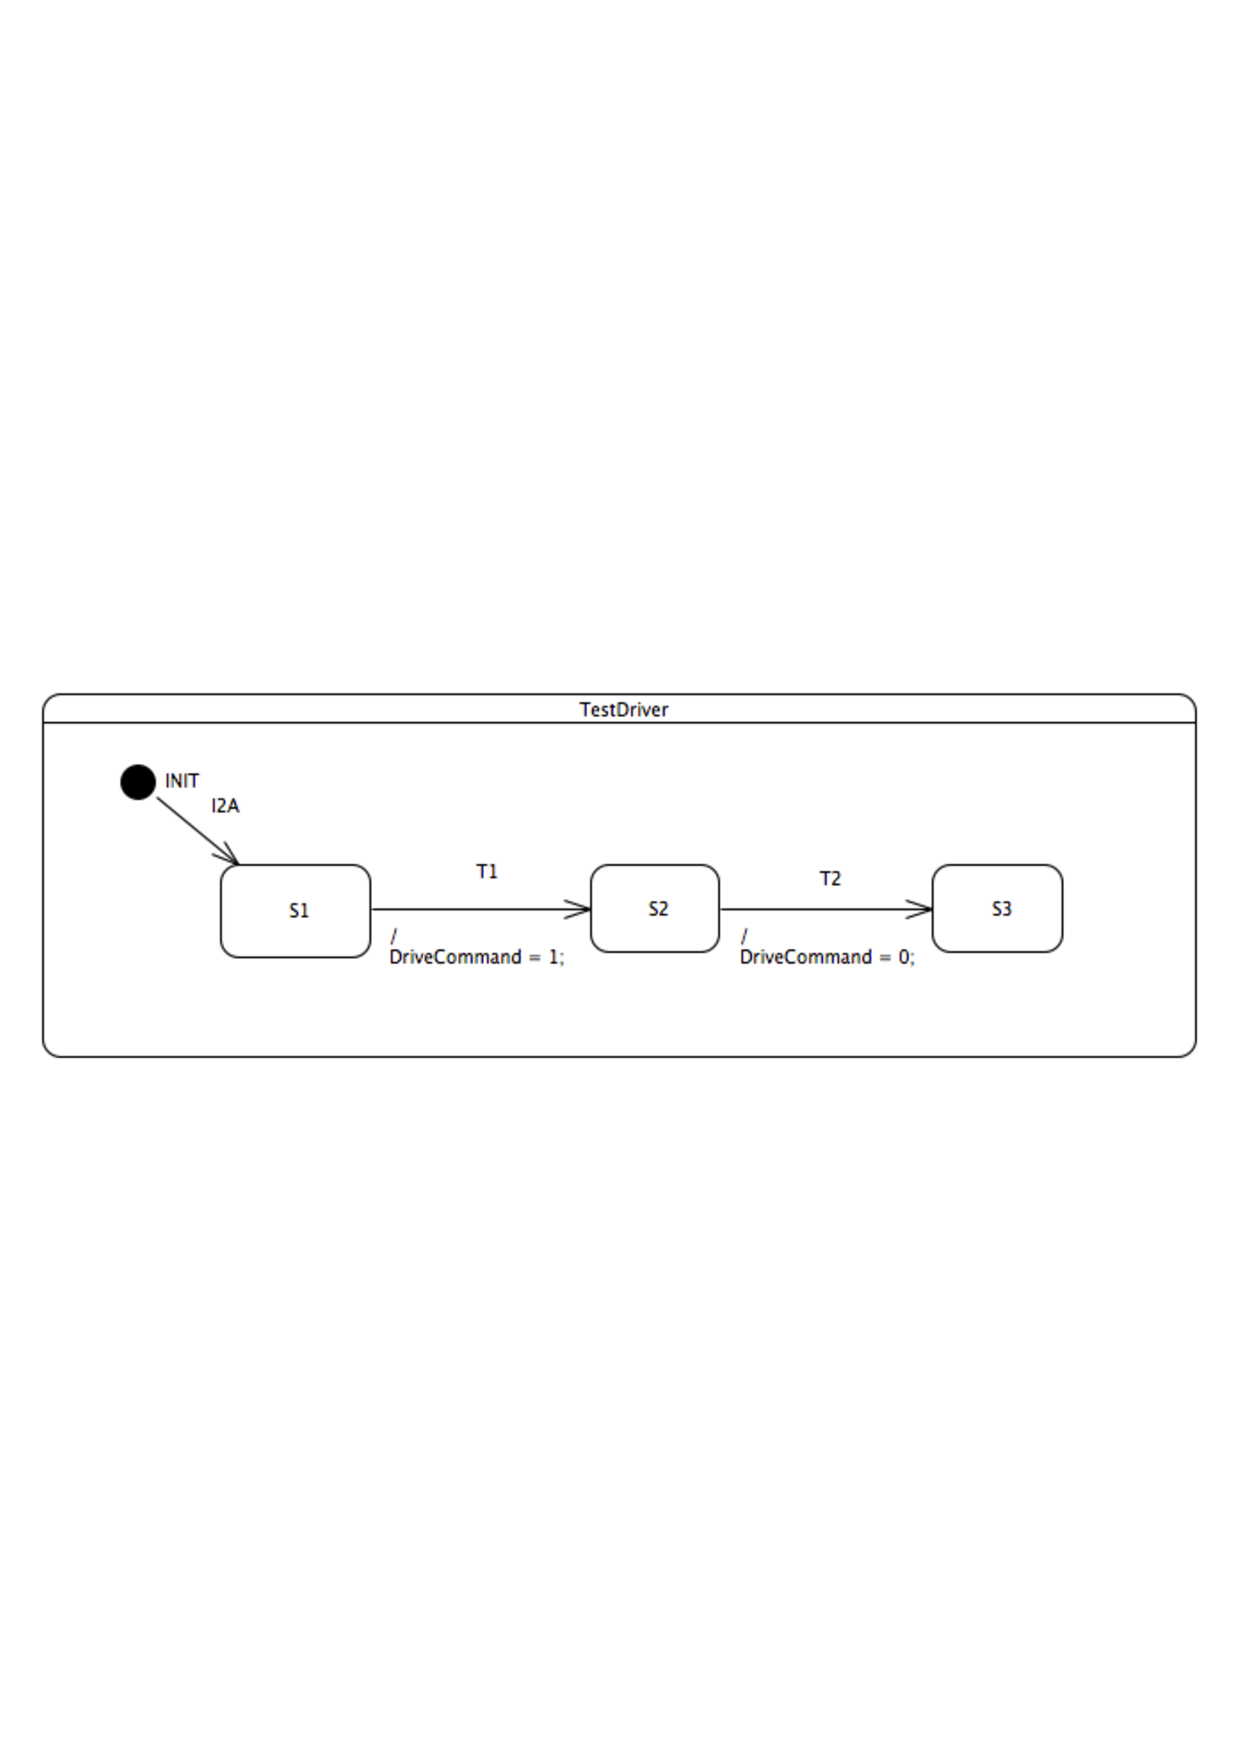
\includegraphics[height=0.8\textheight]{figures/driver}
  \caption{Test Driver Model}
  \label{fig:driver}
\end{figure}

%************************************************************************
\section{Model Checking the Resulting TTS}
\label{sec:space}
%************************************************************************
We provide two verification scenarios for testing the formal system
obtained from the transformation of the CSM model. Each scenario is
available as a TTS "file" (actually a folder called tpn.tts) inside
the 05-Work folder.

\subsection{Scenario 1}
Scenario 1 includes the following initial values for the parameters:
\begin{itemize}
\item
SimulatedTrainSpeed = 110
\item
V\_mrsp = 120
\item
SBAvailable = true
\item
DriveCommand = 1. The initial drive command is acceleration. 
\item
T1 transition in Driver model has an effect behavior DriveCommand = 1. The time duration for the initial behavior (acceleration) is 20000. 
\item
T2 transition in Driver model has an effect behavior DriveCommand = 0. The time duration for the behavior before keeping speed (acceleration) is 10000. 
\end{itemize}

We give in the table below the number of reachable states (or
markings) of the resulting TPN. A marking is defined by a particular
value for each system variable and for each internal state of the
blocks. This gives a rough idea of the complexity of checking
reachability properties on the system. "Classes" take into account
timing constraints on top of the markings; hence there is always more
classes than markings. The generation of the whole state space takes
for Scenario 1 takes
less than 24 seconds (system time: 23.350s).\\

\begin{center}
  \begin{tabular}{|c|c|c|c|}
    \hline
    markings & domains & classes & transitions \\
    \hline
    399 & 455880 & 456926 & 978970 \\ 
    \hline
  \end{tabular}
\end{center}

\subsection{Scenario 2}
Scenario 2 includes the following initial values of parameters:
\begin{itemize}
\item
SimulatedTrainSpeed = 0
\item
V\_mrsp = 160
\item
SBAvailable = true
\item
DriveCommand = 1. The initial drive command is acceleration. 
\item
T1 transition in Driver model has an effect behavior DriveCommand = 2. The time duration for initial behavior (acceleration) is 200000. 
\item
T2 transition in Driver model has an effect behavior DriveCommand = 0. The time duration for the behavior before keeping speed (deceleration) is 100000. 
\end{itemize}

The size of the state graph for scenario 2 is shown in the table
below. The generation of the whole state space takes less than 26s
(system time of 25.912s).

\begin{center}
  \begin{tabular}{|c|c|c|c|}
    \hline
    markings & domains & classes & transitions \\
    \hline
    474 & 700129	 & 700472 & 1201679 \\ 
    \hline
  \end{tabular}
\end{center}

%************************************************************************
\section{Verification of Requirements}
\label{sec:verif}
%************************************************************************

We have used our model-checking toolbox to check the properties stated
in the work by Univ. Bremen~\cite{csmwp4}. These properties are a
direct translation into temporal logic of the requirements found on
the Subset 026 documents. Since the CSM model does not take into
account the possible activation and de-activation of the CSM, we have
not dealt with three requirements. (By default, the CSM is always
activated.) We provide an interpretation of the nine remaining
requirements using LTL, see Table \ref{tab:reqltl}. To simplify the
the LTL formula, we have used simple names for naming the relevant
variables. Full names, integrating information on the hierarchy,
should be used when model-checking the actual systems in Tina.


\begin{table}[ht!]
\footnotesize
	\caption{LTL}
	\begin{center}
    \begin{tabular}{|c|p{10cm}|}
    \hline
	Requirement & LTL Formula \\
	\hline
	\hline
	req\_01 & EmergencyBrakeCommand $\wedge$ SBAvailable=0 $\wedge$ SimulatedTrainSpeed <= V\_mrsp $\wedge$  RevocationEmergencyBrake=0\\
	\hline
	req\_02 & ServiceBrakeCommand $\wedge$ SBAvailable=0 $\wedge$ SimulatedTrainSpeed <= V\_mrsp\\
	\hline
	req\_03 & ServiceBrakeCommand $\wedge$ SBAvailable=0 $\wedge$ SimulatedTrainSpeed gt (V\_mrsp + dV\_sbi) $\wedge$ SimulatedTrainSpeed lt (V\_mrsp + dV\_ebi) \\
	\hline
	req\_08 &  $\diamond$ ((NORMAL	 $\wedge$ SimulatedTrainSpeed <= V\_mrsp) U (NORMAL $\wedge$ SimulatedTrainSpeed gt V\_mrsp + dV\_warning $\wedge$ SimulatedTrainSpeed <= V\_mrsp + dV\_sbi)) \\
	\hline
	req\_09 & $\diamond$ ((NORMAL $\wedge$ SimulatedTrainSpeed <= V\_mrsp) $\wedge$ ((NORMAL $\wedge$ SimulatedTrainSpeed <= V\_mrsp) U (NORMAL $\wedge$ SimulatedTrainSpeed gt V\_mrsp + dV\_sbi $\wedge$ SimulatedTrainSpeed <= V\_mrsp + dV\_ebi))) \\
	\hline
	req\_10 & $\diamond$ ((NORMAL $\wedge$ SimulatedTrainSpeed <= V\_mrsp) $\wedge$ ((NORMAL $\wedge$ SimulatedTrainSpeed <= V\_mrsp) U (NORMAL $\wedge$ SimulatedTrainSpeed gt V\_mrsp + dV\_sbi)))\\
	\hline
	req\_11 & $\diamond$ ((OVERSPEED $\wedge$ SimulatedTrainSpeed <= V\_mrsp) $\wedge$ ((OVERSPEED $\wedge$ SimulatedTrainSpeed <= V\_mrsp) U (NORMAL $\wedge$ SimulatedTrainSpeed gt V\_mrsp + dV\_sbi $\wedge$ SimulatedTrainSpeed <= V\_mrsp + dV\_ebi))) \\
	\hline
	req\_12 & $\diamond$ ((OVERSPEED $\wedge$ SimulatedTrainSpeed <= V\_mrsp) $\wedge$ ((OVERSPEED $\wedge$ SimulatedTrainSpeed <= V\_mrsp) U (NORMAL $\wedge$ SimulatedTrainSpeed gt V\_mrsp + dV\_sbi))) \\
	\hline
	req\_13 & $\diamond$ ((WARNING $\wedge$ SimulatedTrainSpeed <= V\_mrsp) $\wedge$ ((WARNING $\wedge$ SimulatedTrainSpeed <= V\_mrsp) U (WARNING $\wedge$ SimulatedTrainSpeed gt V\_mrsp + dV\_ebi))) \\
	\hline
    \end{tabular}
    \end{center}
\label{tab:reqltl}
\end{table} 

%%% Local Variables: 
%%% mode: latex
%%% TeX-master: "csm"
%%% End: 
